\section{Finite-element discretization}

\subsection{Heat pump discretization}

Het algemene model van de warmtepomp en airco wordt afgeleid met behulp van het volgende geschematiseerde black box model:

\subsection{Buffer vessel discretization}

Als voorbeeld van een model met warmtestromen en warmtediffusie wordt het volgende model van
een buffervat beschouwd:

\begin{figure}[H]
	\centering
	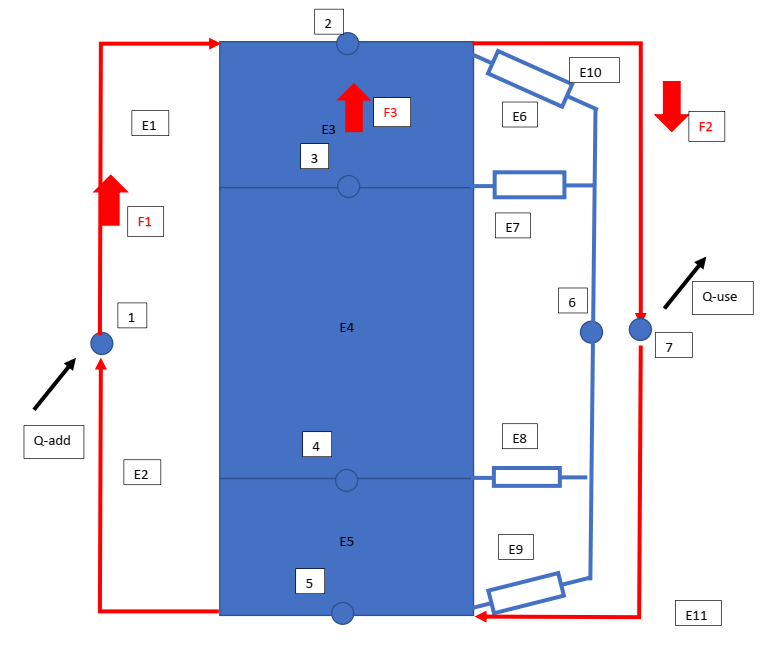
\includegraphics[width=0.7\columnwidth]{Figures/FEwatervat.png}
	\caption[Short title]{Finite-element buffer vessel}
	\label{fig:FEbuffervessel}
\end{figure}

Dit is een buffervat in een verwarmingsinstallatie.

Voor het modelleren hiervan wordt gebruik gemaakt van een tweetal universele elementen:

\begin{enumerate}
	\item Exchange element. Dit element beschrijft warmtetransportt via een vloeistofstroom $F$ door het element en warmtetransport door geleiding. Het element kan een warmtecapaciteit
	hebben.
	\item Een puntbron. Deze bron beschrijft warmteontwikkeling of warmte-onttrekking in een punt.
\end{enumerate}

Het vat is verdeeld in 3 niveaus over de hoogte:
\begin{enumerate}
	\item Bovenzijde vat (element 3)
	\item Midden vat( element 4 )
	\item Onderzijde vat (element 5 )
\end{enumerate}

In het vat is sprake van:
\begin{itemize}
	\item Warmteverlies naar andere temperatuurniveau ’s en naar de omgeving. De
	omgevingstemperatuur in dit model is gegeven door de temperatuur in punt 7.
	De elementen die het volume van het vat beschrijven (E3,E4 en E5) wisselen warmte uit naar
	elkaar en naar punt 6.
	\item Warmtetransport door waterstromen. In waterstromen buiten het vat wordt warmte
	onttrokken of toegevoegd. In het vat is een waterstroom die zorgt voor het kortsluiten van
	de kringlopen.
\end{itemize}

Deze beide mechanismen worden meegenomen in het model.

Er wordt verondersteld dat gebruik wordt gemaakt van gelaagdheid. Boven in het vat heerst een
hogere temperatuur dan onderin het vat. Daarnaast is er sprake van een tweetal leidingen waarin
warmte wordt uitgewisseld met de omgeving:

\begin{itemize}
	\item Een leiding waarin warmte wordt toegevoegd aan het vat $\dot{Q}_{add}$. Deze leiding neemt
	vloeistof (water) onder uit het vat (punt 5), verhoogt de temperatuur door warmte-inbreng
	(punt 1) en brengt het water boven in het vat weer in. Deze leiding bestaat uit de
	elementen E1 (boven) en E2 (onder). In deze leiding is een vloeistofstroom $F_1 (kJ/(K·s))$
	aanwezig die de warmte transporteert.
	\item Een leiding waarin warmte wordt onttrokken aan het vat $\dot{Q}_{use}$. Deze leiding neemt vloeistof (water) boven uit het vat (punt 2), verlaagt de temperatuur door warmteonttrekking (punt 7) en brengt het water boven in het vat weer in. Deze leiding bestaat uit	de elementen E10 (boven) en E11 (onder). In deze leiding is een vloeistofstroom $F_2 (kJ/(K·s))$ aanwezig die de warmte transporteert.
\end{itemize}

\subsection{Matrixvergelijking}

Voor het oplossen van de temperatuurverdeling wordt per knooppunt een energiebalans opgesteld.
Deze energiebalans resulteert in een matrixvergelijking.

\begin{equation}
	\begin{aligned}
	    \mathbf{K \theta + C \dot{\theta}} = \mathbf{\dot{q}}	    	
	\end{aligned}
\end{equation}

$K$: de warmtegeleidingsmatrix (W/K)
$C$: de warmtecapaciteitsmatrix (J/K)
$\theta$: de temperatuursvector (K)
$\dot{\theta}$: de tijdsafgeleide van de temperatuursvector (K/s)
$\dot{q}$: de vector met thermische brontermen (W)

\subsection{Elementen in de stroming}

Om te komen tot het matrixmodel wordt begonnen met één exchange element zoals hierboven
geïntroduceerd (E1,E2,E3,E4,E5,E10,E11). Dit element bevat 2 knooppunten. De volgende veronderstellingen worden gedaan:

\begin{itemize}
	\item Het element bevat 2 knooppunten waarmee deze verbonden is met de omgeving. De
	nummering bedraagt: $n_1$ en $n_2$.
	\item Binnen het element heerst een lineair verlopende temperatuur, van knooppunt naar
	knooppunt.
	\item Binnen het element is een vloeistofstroom $F$ die zorgt voor additioneel warmtetransport. De stroomrichting is van knooppunt 1 naar knooppunt 2.
	\item De warmtecapaciteit van het element wordt evenredig verdeeld over de knooppunten.
\end{itemize}

De warmtestroom vanuit het element naar knoopunten 1 en 2 moet in balans zijn met de andere
warmtestromen en de warmtegeneratie in de betreffende knooppunten.

\begin{figure}[H]
	\centering
	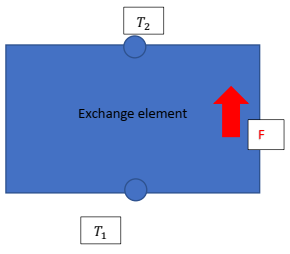
\includegraphics[width=0.7\columnwidth]{Figures/exchange_element.png}
	\caption[Short title]{Exchange element buffer vessel}
	\label{fig:exchange_element}
\end{figure}

Voor de warmtestromen vanaf knooppunt 1 geldt:

\begin{equation}
	\begin{aligned}
		(T_1 - T_2) \cdot \frac{1}{R_e} + C_{e1,1} \cdot \frac{dT_1}{dT} = \dot{Q}_{ext,1}	    	
	\end{aligned}
\end{equation}

$T_1$: temperatuur in knooppunt 1 \\
$T_2$: temperatuur in knooppunt 2 \\
$R_e$: warmteweerstand voor geleiding tussen knooppunt 1 en 2 \\
$C_{e1,1}$: warmtecapaciteit in knooppunt 1 van element 1 \\
$\frac{dT_1}{dT}$: temperatuursverandering in de tijd in knooppunt 1 \\
$\dot{Q}_{ext,1}$: externe warmtetoevoer in knooppunt 1 \\

De vloeistofstroom $F$ vanuit knooppunt $T_1$ heeft dezelfde temperatuur als $T_1$ en heeft dus geen invloed op de temperatuur in $T_1$.

Voor de warmtestromen vanaf punt 2 geldt:

\begin{equation}
	\begin{aligned}
		(T_2 - T_1) \cdot \frac{1}{R_e} + F \cdot (T_2 - T_1) + C_{e1,2} \cdot \frac{dT_2}{dT} = \dot{Q}_{ext,2}	    	
	\end{aligned}
\end{equation}

$C_{e1,2}$: warmtecapaciteit in knooppunt 2 van element 1 \\
$\frac{dT_2}{dT}$: temperatuursverandering in de tijd in knooppunt 2 \\
$\dot{Q}_{ext,2}$: externe warmtetoevoer in knooppunt 2 \\

In matrixnotatie:

\begin{equation}
	\begin{aligned}
	\begin{bmatrix}
	    1/R_e & -1/R_e \\
	    -1/R_e -F &  1/R_e + F
    \end{bmatrix}
    \cdot
    \begin{bmatrix}
    	T_1 \\
    	T_2
    \end{bmatrix}
    +
    	\begin{bmatrix}
    	C_{e1,1} & 0 \\
    	0 &  C_{e1,2}
    \end{bmatrix}
    \cdot
    \begin{bmatrix}
    	\frac{dT_1}{dt} \\
	    \frac{dT_2}{dt}
    \end{bmatrix}	
    =
        \begin{bmatrix}
    	\dot{Q}_{ext,1} \\
    	\dot{Q}_{ext,2}
    \end{bmatrix}  	
	\end{aligned}
\end{equation}

Merk op dat door de aanwezigheid van een vloeistofstroom $F$, de geleidingsmatrix niet langer symmetrisch is.

Daarnaast wordt gebruik gemaakt van elementen die alleen een warmteweerstand weergeven. Deze
elementen (E6,E7,E8 en E9) kunnen worden gerepresenteerd met de volgende matrixvergelijking

\begin{equation}
	\begin{aligned}
		\begin{bmatrix}
			1/R_e & -1/R_e \\
			-1/R_e &  1/R_e
		\end{bmatrix}
		\cdot
		\begin{bmatrix}
			T_1 \\
			T_2
		\end{bmatrix}	
		=
		\begin{bmatrix}
			\dot{Q}_{ext,1} \\
			\dot{Q}_{ext,2}
		\end{bmatrix}  	
	\end{aligned}
\end{equation}

\subsection{Systemmmatrices van het buffervat}

Er wordt nu een systeemmatrix opgesteld voor het schematisch weergegeven model. Deze
systeemmatrix wordt opgebouwd uit de verschillende elementmatrices. De noodzakelijke rang van
deze systeemmatrix is het aantal knooppunten in het warmtestroomschema minus het aantal
voorgeschreven knooppunten in dit schema. Er zijn 7 knooppunten in het model. In dit geval wordt
in punt 6 de temperatuur voorgeschreven.
Er resteren dan 6 onafhankelijke vrijheidsgraden.

\subsubsection{Capaciteitsmatrix $\mathbf{C}$}

There are 7 nodes in the system. The heat capacities are:

\begin{equation}
	\begin{aligned}
\text{node 1} & \quad C_{e1,1} + C_{e2,2} = 0.5 \cdot (C_{e1} + C_{e2})\\
\text{node 2} & \quad C_{e1,2} + C_{e3,1} + C_{e10,2} + C_{e6,2} = 0.5 \cdot (C_{e1} + C_{e3} + C_{e10} + C_{e6}) \\
\text{node 3} & \quad C_{e3,2} + C_{e4,1} + C_{e7,2} = 0.5 \cdot (C_{e3} + C_{e4} + C_{e7}) \\
\text{node 4} & \quad C_{e4,2} + C_{e5, 1} + C_{e8,2} = 0.5 \cdot (C_{e4} + C_{e5} + C_{e8}) \\
\text{node 5} & \quad C_{e5,2} + C_{e2, 1} + C_{e9, 2} + C_{11,2} = 0.5 \cdot (C_{e5} + C_{e2} + C_{e9} + C_{11}) \\
\text{node 6} & \quad C_{e6,1} + C_{e7, 1} +  C_{e8, 1} +  C_{e9, 1} = 0.5 \cdot (C_{e6} + C_{e7} +  C_{e8} +  C_{e9}) \\
\text{node 7} & \quad C_{e10,2} + C_{e11,1} = 0.5 \cdot (C_{e10} + C_{e11})
	\end{aligned}
\end{equation}

\begin{tiny}
\[
0.5 \cdot 
\begin{bmatrix}
	C_{e1} + C_{e2} & 0 & 0 & 0 & 0 & 0 & 0 \\
	0 & C_{e1} + C_{e3} + C_{e10} + C_{e6} & 0 & 0 & 0 & 0 & 0 \\
	0 & 0 & C_{e3} + C_{e4} + C_{e7} & 0 & 0 & 0 & 0 \\
	0 & 0 & 0 & C_{e4} + C_{e5} + C_{e8} & 0 & 0 & 0 \\
	0 & 0 & 0 & 0 & C_{e5} + C_{e2} + C_{e9} + C_{e11} & 0 & 0 \\
	0 & 0 & 0 & 0 & 0 & C_{e6} + C_{e7} +  C_{e8} + C_{e9} & 0 \\
	0 & 0 & 0 & 0 & 0 & 0 & C_{e10} + C_{e11}
\end{bmatrix}
\]
\end{tiny}

The heat capacities of element E1, E2, E10 and E11 (pipelines) are very small and can be approximated to be zero. Also, the elements E6, E7, E8 and E9 are thermal leaks, connected to node 6, which may be a boundary condition.

The capacity matrix thus reduces to:

\[
0.5 \cdot 
\begin{bmatrix}
	\approx 0 & 0 & 0 & 0 & 0 & 0 & 0 \\
	0 & C_{e3} & 0 & 0 & 0 & 0 & 0 \\
	0 & 0 & C_{e3} + C_{e4} & 0 & 0 & 0 & 0 \\
	0 & 0 & 0 & C_{e4} + C_{e5} & 0 & 0 & 0 \\
	0 & 0 & 0 & 0 & C_{e5} & 0 & 0 \\
	0 & 0 & 0 & 0 & 0 & 0 & 0 \\
	0 & 0 & 0 & 0 & 0 & 0 & \approx 0
\end{bmatrix}
\]

In the approximation above, the buffer vessel system is not solvable, without adding some heat capacity to nodes N1 and N7. \emph{e.g.} these nodes must be coupled with a house model element with finite heat capacity.

In any case, the node N6 (boundary condition) does not contribute a DOF to the system of equations. Row 6 and column 6 will be removed from the set of equations.

\lstinputlisting[label=lst:cmatrix, linerange={52-86}, 
caption={Generation of capacity matrix}] 
{../../housemodel/finite\_elements/ckf\_elements\_xl.py}

\subsubsection{$\mathbf{\dot{q}}$-vector}

De vector $\mathbf{\dot{q}}$ wordt gegeven door:

\[
\left(\hspace{-5pt}\begin{array}{cc|c}
	1 & 1 & \dot{q}_1 = \dot{Q}_{add}\\
	2 & 2 & \dot{q}_2\\
	3 & 3 & \dot{q}_3\\
	4 & 4 & \dot{q}_4\\
	5 & 5 & \dot{q}_5\\
	6 & 6 & \dot{q}_6\\
	7 & 7 & \dot{q}_7 = -\dot{Q}_{use}
\end{array}\hspace{-5pt}\right)
\]

\[
\left(\hspace{-5pt}\begin{array}{cc|c}
	1 & 2 & 3 \\
	4 & 5 & 9
\end{array}\hspace{-5pt}\right)
\]

In nodes N1 and N7 an external een heat source / heat sink is contributing to the power balance.

Het voorgeschreven knooppunt (randvoorwaarde, boundary condition) 6 is verbonden aan knooppunten 2, 3, 4 en 5. Dit zijn de ook de vrijheidsgraden 2, 3, 4 en 5. Vrijheidsgraden worden aangegeven met DOF (degree of freedom). In de overeenkomstige knooppunten wordt de capaciteits? stiffness matrix $\mathbf{K}$ en de bronvector (load vector) $\mathbf{\dot{q}}$ aangepast.De aanpassing van de K-matrix wordt verderop toegelicht. De bronvector wordt als volgt aangepast:

\[
\begin{bmatrix}
	1 & 1 & \dot{Q}_{add} \\
	2 & 2 & 0 - \frac{1}{R_{2,6}} \\
	3 & 3 & 0 - \frac{1}{R_{3,6}} \\
	4 & 4 & 0 - \frac{1}{R_{4,6}} \\
	5 & 5 & 0 - \frac{1}{R_{5,6}} \\
	6 & 7 & -\dot{Q}_{use}
\end{bmatrix}
\]


\subsubsection{Geleidingsmatrix $\mathbf{K}$}

elements with heat capacity must have two nodes:
E3, E4, E5

elements without heat capacity have two nodes as well:
E1, E2, E6, E7, E8, E9, E10, E11

elements without heat conduction:
E1, E2, E10, E11

elements with heat conduction:
E3, E4, E5, E6, E7, E8, E9

elements with heat convection (flow):
E1, E2, E3, E4, E5, E10, E11

The "conduction" matrix is equivalent to the stiffness matrix in a mechanical FE analysis.
In terms of the thermal system topology this matrix contains the "edges" between the nodes. The matrix is setup as a 7 x 7 square zero matrix with the nodes as DOF.

\begin{equation}
	\begin{aligned}
		\begin{bmatrix}
			0 & 0 & 0 & 0 & 0 & 0 & 0\\
			0 & 0 & 0 & 0 & 0 & 0 & 0\\
			0 & 0 & 0 & 0 & 0 & 0 & 0\\
			0 & 0 & 0 & 0 & 0 & 0 & 0\\
			0 & 0 & 0 & 0 & 0 & 0 & 0\\
			0 & 0 & 0 & 0 & 0 & 0 & 0\\
			0 & 0 & 0 & 0 & 0 & 0 & 0\\
		\end{bmatrix}
	\end{aligned}
\end{equation}

The conductive elements in the system are:

\begin{equation}
	\begin{aligned}
        \frac{1}{R_{2,3}} & = & \frac{1}{R_{e3}} \\
        \frac{1}{R_{3,4}} & = & \frac{1}{R_{e4}} \\
        \frac{1}{R_{4,5}} & = & \frac{1}{R_{e5}} \\
        \frac{1}{R_{2,6}} &  & \frac{1}{R_{3,6}} & & \frac{1}{R_{4,6}} & & \frac{1}{R_{5,6}} 
	\end{aligned}
\end{equation}

The conductive element $\frac{1}{R_{12}} = \frac{1}{R_{e1}} = 0$. This means $R_{12} \rightarrow \infty$. We assume, the pipeline is perfectly insulated and creates no heat leak. Thermal energy flowing \emph{through} it is completely delivered to the target node. Likewise, this holds for the elements E2, E10 and E11.

\begin{equation}
	\begin{aligned}
		\begin{bmatrix}
			0 & 0 & 0 & 0 & 0 & 0 & 0\\
            0 & 0 & \frac{-1}{R_{2,3}} & 0 & 0 & \frac{-1}{R_{2,6}} & 0 \\
            0 & \frac{-1}{R_{2,3}} & 0 & \frac{-1}{R_{3,4}} & 0 & \frac{-1}{R_{3,6}} & 0\\
            0 & 0 & \frac{-1}{R_{3,4}} & 0 & \frac{-1}{R_{4,5}} & \frac{-1}{R_{4,6}} & 0\\
            0 & 0 & 0 & \frac{-1}{R_{4,5}} & 0 & \frac{-1}{R_{5,6}} & 0 \\
            0 & \frac{-1}{R_{2,6}} & \frac{-1}{R_{3,6}} & \frac{-1}{R_{4,6}} & \frac{-1}{R_{5,6}} & 0 & 0\\
            0 & 0 & 0 & 0 & 0 & 0 & 0\\
		\end{bmatrix}
	\end{aligned}
\end{equation}

\begin{equation}
	\begin{aligned}
		\begin{bmatrix}
			0 & 0 & 0 & 0 & 0 & 0 & 0 \\
			0 & \frac{1}{R_{2,3}} + \frac{1}{R_{2,6}} & \frac{-1}{R_{2,3}} & 0 & 0 & \frac{-1}{R_{2,6}} & 0 \\
			0 & \frac{-1}{R_{2,3}} & \frac{1}{R_{2,3}} + \frac{1}{R_{3,4}} + \frac{1}{R_{3,6}} & \frac{-1}{R_{3,4}} & 0 & \frac{-1}{R_{3,6}} & 0 \\
			0 & 0 & \frac{-1}{R_{3,4}} & \frac{1}{R_{3,4}} +  \frac{1}{R_{4,5}} + \frac{1}{R_{4,6}} & \frac{-1}{R_{4,5}} & \frac{-1}{R_{4,6}} & 0\\
			0 & 0 & 0 & \frac{-1}{R_{4,5}} & \frac{1}{R_{4,5}} + \frac{1}{R_{5,6}} & \frac{-1}{R_{5,6}} & 0 \\
			0 & \frac{-1}{R_{2,6}} & \frac{-1}{R_{3,6}} & \frac{-1}{R_{4,6}} & \frac{-1}{R_{5,6}} & \frac{1}{R_{2,6}} + \frac{1}{R_{3,6}} +  \frac{1}{R_{4,6}} + \frac{1}{R_{5,6}} & 0\\
			0 & 0 & 0 & 0 & 0 & 0 & 0\\
		\end{bmatrix}
	\end{aligned}
\end{equation}

If node N6 is a boundary condition \emph{i.e.} $T_6$ is given as a constant. The corresponding row in the $\mathbf{K}$ and $\mathbf{C}$ matrices can be removed. For the nodes that are connected to node N6 (row 2, 3, 4 and 5) the thermal connection can be moved to the $\mathbf{\dot{q}}$ vector. This can be seen by writing down the differential equation for node N2:

\begin{equation}
	\begin{aligned}
        0.5 \, C_{e3} \cdot \frac{dT_2}{dt} = \frac{1}{R_{2,3}} (T_3 - T_2) + \frac{1}{R_{2,6}} (T_6 - T_2) & = (-\frac{1}{R_{2,3}} - \frac{1}{R_{2,6}}) \cdot T_2 + \frac{1}{R_{2,3}} \cdot T_3 + \frac{1}{R_{2,6}} \cdot T_6 
	\end{aligned}
\end{equation}

\begin{equation}
	\begin{aligned}
        \mathbf{K \theta} \qquad & + & \mathbf{C \dot{\theta}} & = & \mathbf{\dot{q}} \\
		(\frac{1}{R_{2,3}} + \frac{1}{R_{2,6}}) \cdot T_2 - \frac{1}{R_{2,3}} \cdot T_3 \; & + & 0.5 \, C_{e3} \cdot \frac{dT_2}{dt} & = & \frac{1}{R_{2,6}} \cdot T_6
	\end{aligned}
\end{equation}

\textbf{Note:} the sum of each row in $\mathbf{K}$ is not \emph{zero} anymore, but equals the corresponding vector element in $\mathbf{\dot{q}}$.

This reduces the matrices to:

\begin{equation}
	\begin{aligned}
		\mathbf{C} & =
		0.5 \cdot 
		\begin{bmatrix}
			\approx 0 & 0 & 0 & 0 & 0 & 0 \\
			0 & C_{e3} & 0 & 0 & 0 & 0 \\
			0 & 0 & C_{e3} + C_{e4} & 0 & 0 & 0 \\
			0 & 0 & 0 & C_{e4} + C_{e5} & 0 & 0 \\
			0 & 0 & 0 & 0 & C_{e5} & 0 \\
			0 & 0 & 0 & 0 & 0 & \approx 0 \\
		\end{bmatrix} \\
        \mathbf{K} & =
			\begin{bmatrix}
				0 & 0 & 0 & 0 & 0 & 0 \\
				0 & \frac{1}{R_{2,3}} + \frac{1}{R_{2,6}} & \frac{-1}{R_{2,3}} & 0 & 0 & 0 \\
				0 & \frac{-1}{R_{2,3}} & \frac{1}{R_{2,3}} + \frac{1}{R_{3,4}} + \frac{1}{R_{3,6}} & \frac{-1}{R_{3,4}} & 0 & 0 \\
				0 & 0 & \frac{-1}{R_{3,4}} & \frac{1}{R_{3,4}} +  \frac{1}{R_{4,5}} + \frac{1}{R_{4,6}} & \frac{-1}{R_{4,5}} & 0\\
				0 & 0 & 0 & \frac{-1}{R_{4,5}} & \frac{1}{R_{4,5}} + \frac{1}{R_{5,6}} & 0 \\
				0 & 0 & 0 & 0 & 0 & 0\\
		\end{bmatrix} \\
        \mathbf{\dot{q}} & =
	        \begin{bmatrix}
		        \dot{Q}_{add} \\
		        \frac{1}{R_{2,6}} \cdot T_6 \\
		        \frac{1}{R_{3,6}} \cdot T_6 \\
		        \frac{1}{R_{4,6}} \cdot T_6 \\
		        \frac{1}{R_{5,6}} \cdot T_6 \\
		        -\dot{Q}_{use}
	        \end{bmatrix}
	\end{aligned}
	\label{eq:CKq_buffer}
\end{equation}

\lstinputlisting[label=lst:kmatrix, linerange={89-113}, 
caption={Generation of stiffness matrix}] 
{../../housemodel/finite\_elements/ckf\_elements\_xl.py}
	
nodes:
E1 has 1 and 2\\
E2 has 1 and 5\\
E3 has 2 and 3\\
E4 has 3 and 4\\
E5 has 4 and 5\\
E6 has 2 and 6\\
E7 has 3 and 6\\
E8 has 4 and 6\\
E9 has 5 and 6\\
E10 has 2 and 7\\
E11 has 5 and 7\\

edges conductivity R and convection F:

1 and 2\\
1 and 5\\
2 and 3\\
3 and 4\\
4 and 5\\
2 and 6\\
3 and 6\\
4 and 6\\
5 and 6\\
2 and 7\\
5 and 7\\


\subsection{Water flow heat transfer}
In the buffer vessel model, cf. Figure \ref{fig:FEbuffervessel}, two water flows run through the system. The first, labeled with $F1$, draws cold water from the bottom layer of the tank. This water is heated up in node 1. In the figure this is done using the external heat flow $Q_{add}$, but in a full system model another model component, for example a heat pump, can be connected here. (\emph{Note}: In order to be able to add heat in a sensible way to the system node 1 has to have some heat capacity. The approximation done above making the capacity of the pipes zero is then not valid.) 
The heated water flows back into the vessel in the top level. The water flow $F1$ outside the vessel, induces an equal sized flow of water in side the vessel from the top layer towards the bottom, through the elements $E3$, $E4$ and $E5$. 

The second water flow $F2$ draws water from the hot top layer. In node 7 a heat flow $Q_{use}$ is extracted. Here, similar to node 1, another model component (for example a radiator) may be connected. (\emph{Note}: the note made for node 1 is valid here is well). 
The cooled water will flow back into the vessel in the bottom layer. F2 induces a flow in the buffer vessel opposite to $F1$, running though $E5$, $E4$ and $E3$,  consecutively. 

The water flows will be controlled by pumps, either by a on/off manner (switching between a fixed water volume per second and 0) or a more advanced varying flow rate. 
Since $F1$ and $F2$ can be controlled separately, the flow in the vessel, labeled with $F3$ can run either direction, from bottom to top, or from top to bottom. The size of the flow $F3$ is given by: $F3 = F1 - F2$. When $F3$ is positive it flows from top to bottom in the vessel. A negative value, implies a water flow from bottom to top. 


\subsubsection{Setting up the flow matrix}\label{s:flow_matrices}
As indicated earlier, the flow rates can be controlled, and thus may change over time. This means that the terms for the heat exchange due to the water flows need to be generated at each time step, or at least after each change in the flow rates. A matrix that represents the flows may be generated in the following process.

\begin{itemize}
	\item First of all, the flows in the system need to be defined in the input file. For each flow we need to know the order it traverses the elements in the system, and more specifically the nodes it passes. This can be done by considering each flow separately, and listing the nodes you pass in the direction of the flow.
	For $F1$ this gives Nodes$_{F1}\left[0, 1, 2, 3, 4, 0 \right]$, and for $F2$ this gives Nodes$_{F2}\left[6,4,3,2,1,6\right]$. (note the labeling of the nodes used here is the number in Figure \ref{fig:FEbuffervessel} minus one.) In the list the first element is equal to the last element, which shows that the flow is a closed loop. The depicted flow $F3$ is only the difference between $F1$ and $F2$, and does not need to be defined by itself. 
	\item From the ordered list of nodes, we can create a "`directed-flow-matrix"' ($\mathbf{DF}$) for each flow. This matrix should be of the same size as the conductance-matrix ($\mathbf{K}$) and the capacity-matrix ($\mathbf{C}$).  The directed-flow-matrix contains a 1 for each matrix-element that corresponds to a connection between nodes in the direction of the flow, and -1 for a connection between nodes in the opposite direction. Thus for flows $F1$ and $F2$ the matrix will be:
	\begin{equation}
		\mathbf{DF_{F1}} = \begin{bmatrix}
							0 & 1 & 0 & 0 & -1& 0 & 0 \\
							-1& 0 & 1 & 0 & 0 & 0 & 0 \\
							0 & -1& 0 & 1 & 0 & 0 & 0 \\
							0 & 0 & -1& 0 & 1 & 0 & 0 \\
							1 & 0 & 0 & -1& 0 & 0 & 0 \\
							0 & 0 & 0 & 0 & 0 & 0 & 0 \\
							0 & 0 & 0 & 0 & 0 & 0 & 0 
							\end{bmatrix}
	\label{eq:DFflow1}
	\end{equation}
	
	\begin{equation}
		\mathbf{DF_{F2}} = \begin{bmatrix}
							0 & 0 & 0 & 0 & 0 & 0 & 0 \\
							0 & 0 & -1& 0 & 0 & 0 & 1 \\
							0 & 1 & 0 & -1& 0 & 0 & 0 \\
							0 & 0 & 1 & 0 & -1& 0 & 0 \\
							0 & 0 & 0 & 1 & 0 & 0 & -1 \\
							0 & 0 & 0 & 0 & 0 & 0 & 0 \\
							0 & -1& 0 & 0 & 1 & 0 & 0 
							\end{bmatrix}
	\label{eq:DFflow1}
	\end{equation}
	
These matrices can be build up from the list as defined in the previous step, by looping through the list and taking the elements Nodes$(i,i+1)$, and filling in a one at the matrix element (Node$(i)$, Node$(i+1)$). After looping through all these pairs we have filled in all connections in the direction of the flow, $\mathbf{DF^{+1}}$. The connections against the flow, $\mathbf{DF^{-1}}$, are given by: $\mathbf{DF^{-1}} = -1 \cdot (\mathbf{DF^{+1}})^T$. Finally, $\mathbf{DF} = \mathbf{DF^{+1}} + \mathbf{DF^{-1}}$. 
\item In each time step, when the flow sizes have been determined by the control algorithms, each directed-flow-matrix is multiplied by its respected flow size in [$\frac{\text{m}^3}{\text{s}}$]. All resulting matrices can then be added together. Assuming a flow of size $f_1$ and $f_2$ for the flows $F1$ and $F2$, respectively we now get the matrix $\mathbf{SF}$:
\begin{equation}
		\mathbf{SF} = f_1 \cdot \mathbf{DF_{F1}} + f_2 \cdot \mathbf{DF_{F2}} = \begin{bmatrix}
							0   & f_1    & 0       & 0       & -f_1    & 0 & 0 \\
							-f_1& 0      & f_1-f_2 & 0       & 0       & 0 & f_2 \\
							0   & f_2-f_1& 0       & f_1-f_2 & 0       & 0 & 0 \\
							0   & 0      & f_2-f_1 & 0       & f_1-f_2 & 0 & 0 \\
							f_1 & 0      & 0       & f_2-f_1 & 0       & 0 & -f_2 \\
							0   & 0      & 0       & 0       & 0       & 0 & 0 \\
							0   & -f_2   & 0       & 0       & f_2     & 0 & 0 
							\end{bmatrix}
	\label{eq:addflows}
	\end{equation}
\item The heat transfer induced by the flows is only in the direction of the water flow. The correct elements are obtained by taking the $\text{min}(\mathbf{SF},0)$, here we mean for each element in $\mathbf{SF}$ we take the minimum of the respective element and 0. Thus, in the case $f_1>f_2$ the matrix $\mathbf{SF}$ will become:
\begin{equation}
		\text{min}(\mathbf{SF},0) =  \begin{bmatrix}
							0   & 0      & 0       & 0       & -f_1    & 0 & 0 \\
							-f_1& 0      & 0		   & 0       & 0       & 0 & 0 \\
							0   & f_2-f_1& 0       & 0			 & 0       & 0 & 0 \\
							0   & 0      & f_2-f_1 & 0       & 0			 & 0 & 0 \\
							0	  & 0      & 0       & f_2-f_1 & 0       & 0 & -f_2 \\
							0   & 0      & 0       & 0       & 0       & 0 & 0 \\
							0   & -f_2   & 0       & 0       & 0       & 0 & 0 
							\end{bmatrix}
	\label{eq:minSFzero}
	\end{equation}



\item Now, the diagonal elements can be computed. The diagonal elements are equal to minus the sum of the of diagonal elements in its respective row. For the matrix given in equation \ref{eq:minSFzero} this results in the flow matrix $\mathbf{F}$:
\begin{equation}
		\mathbf{F} =  \begin{bmatrix}
							f_1   & 0      & 0       & 0       & -f_1    & 0 & 0 \\
							-f_1& f_1      & 0		   & 0       & 0       & 0 & 0 \\
							0   & f_2-f_1& -(f_2-f_1)       & 0			 & 0       & 0 & 0 \\
							0   & 0      & f_2-f_1 & -(f_2-f_1)       & 0			 & 0 & 0 \\
							0	  & 0      & 0       & f_2-f_1 & f_1      & 0 & -f_2 \\
							0   & 0      & 0       & 0       & 0       & 0 & 0 \\
							0   & -f_2   & 0       & 0       & 0       & 0 & f_2 
							\end{bmatrix}
	\label{eq:flowmatrix}
	\end{equation}

\item Finally, we need to multiply the resulting flow matrix with the density ($\rho_{water}$) and the specific heat ($c_{p, water}$), in order to obtain the heat transferred by the water due to the water flows. The resulting matrix can be added to the K matrix as given in equation \ref{eq:CKq_buffer}.
\end{itemize} 

\begin{equation}
	\begin{aligned}
		v_{pump} \cdot A_{pipe} \cdot \rho_{water} \cdot c_{p, water} =  \qquad \left[ \frac{m}{s} \cdot m^2 \cdot\frac{kg}{m^3} \cdot \frac{J}{kg \cdot K} = \frac{J}{K \cdot s} = \frac{W}{K}\right]
	\end{aligned}
\end{equation}

\emph{Note 1}, when the system contains flows of different fluids, the described steps need to be followed for each fluid type separately. Each fluid will have its own matrix which will contribute to the overall system. This also implies the need to define the density and specific heat for each flow.

\emph{Note 2}, at this moment the process does not deal with splitting and merging of the water flows. Therefore, a system that may control valves to distribute the water over different radiators using one supply pipe, and one pump, is not feasible in this concept, yet.   


\subsection{House model (2R2C-model) in finite element structure}

Although the equations of the house model as presented in Section \ref{s:lumped-element} have a very similar structure, one should not mix the lumped-element approach presented in Section \ref{s:lumped-element} with the finite-element approach of this chapter. Therefore, we revisit the 2R2C-model in order to incorporate the house model in the finite-element approach. 

Recall that, in the lumped-element model, the 2R2C model contained two connected elements with a heat capacity, one for the air in the house and one for the building structure. In the lumped element model these heat capacities cold be directly modeled with one capacitor for the air and one for the walls. The heat transfer between the two capacities was modeled with a single heat conductor (resistor). Finally, the air could exchange heat with the node fro the ambient temperature, which has a fixed temperature. This resulted in the model as presented in Figure \ref{fig:2R2Cagain}. 
\begin{figure}[H]
	\centering
	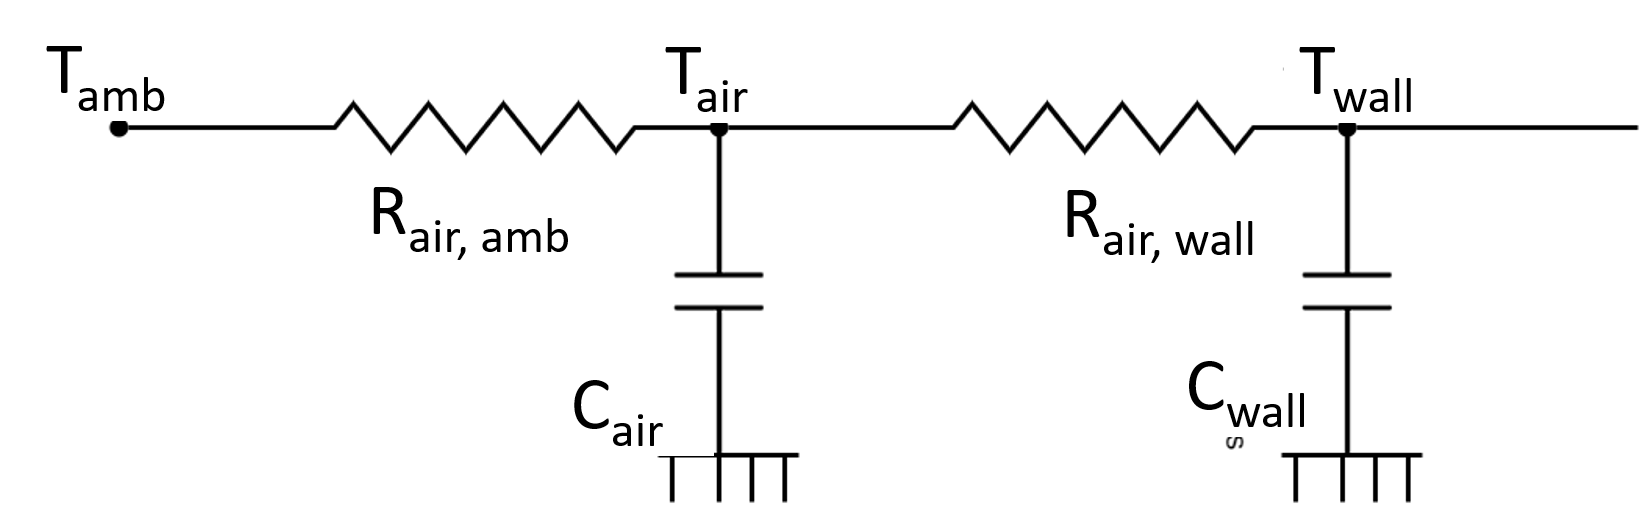
\includegraphics[width=0.7\columnwidth]{Figures/2R2Cmodel_rev.png}
	\caption[Short title]{2R-2C house model revisited}
	\label{fig:2R2Cagain}
\end{figure}

When we want to model this same concept in the finite-element structure, we need four elements: one element that represents the air, one that represents the walls, one element for the interaction between the air and the wall, and one element for the interaction between the air and the ambient surroundings. The model is sketched in Figure \ref{fig:fin-el-house}.
\begin{figure}[H]
	\centering
	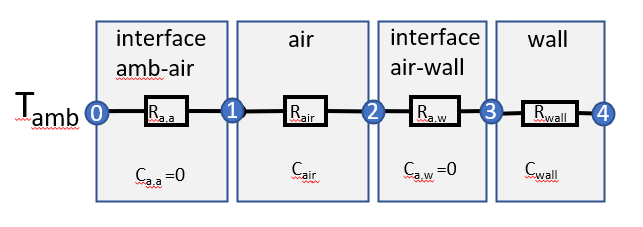
\includegraphics[width=0.7\columnwidth]{Figures/finite_element_house.png}
	\caption[Short title]{Finite element representation of the 2R2C house model}
	\label{fig:fin-elhouse}
\end{figure}

In this model the heat capacity of the air will be divided over the nodes 1 and 2, with $0.5\cdot C_{air}$ for each node. In the same manner, the heat capacity of the wall will be divided over the nodes 3 and 4. The elements that are needed for the heat exchange between air and wall, and air and ambient surroundings do not have any heat capacity. 

In the lumped-element model the air and wall were considered to have a homogeneous temperature. This is no longer the case in the finite element model. Theoretically, one could make the heat resistance within the air and wall elements zero, which would lead to an instantaneous heat transfer between the nodes 1 and 2, and 3 and 4, respectively. Thus resulting in an equal temperature for nodes 1 and 2, and 3 and 4. 
However, computationally this will lead to problems, since the corresponding $\mathbf{K}$ matrix will have $\frac{1}{R} = \infty$  entries in the representative positions. Therefore, in practice, an internal heat resistance has to be applied in the air and wall elements. Thus, resulting in a gradient within the elements. 

The $\mathbf{C}$ and $\mathbf{K}$ matrices of the system will be:
\begin{equation}
	\begin{aligned}
		\mathbf{C} &= \begin{bmatrix}
			0 & 0 & 0 & 0 & 0 \\
			0 & 0.5 \cdot C_{air} & 0 & 0 & 0 \\
			0 & 0 & 0.5 \cdot C_{air} & 0 & 0 \\
			0 & 0 & 0 & 0.5 \cdot C_{wall} & 0 \\
			0 & 0 & 0 & 0 & 0.5 \cdot C_{wall}\\
		\end{bmatrix}\\
	\mathbf{K} &= \begin{bmatrix}
		\frac{1}{R_{a,a}} & -\frac{1}{R_{a,a}} & 0 & 0 & 0 \\
		-\frac{1}{R_{a,a}} & \frac{1}{R_{a,a}}+\frac{1}{R_{air}} & -\frac{1}{R_{air}} & 0 & 0 \\
		0 & -\frac{1}{R_{air}} & \frac{1}{R_{air}}+\frac{1}{R_{a,w}} & -\frac{1}{R_{a,w}} & 0 \\
		0 & 0 & -\frac{1}{R_{a,w}}& \frac{1}{R_{a,w}}+\frac{1}{R_{wall}} & -\frac{1}{R_{wall}} \\
		0 & 0 & 0 & -\frac{1}{R_{wall}} & \frac{1}{R_{wall}} 
		\end{bmatrix}
	\end{aligned}
\label{eq:CK_finel_house}
\end{equation}


%\[
%\begin{bmatrix}
	%1 & 1 & \dot{Q}_{add}\\
	%2 & 2 & 0 - \frac{1}{R_{2,6}}\\
	%3 & 3 & 0 - \frac{1}{R_{3,6}}\\
	%4 & 4 & 0 - \frac{1}{R_{4,6}}\\
	%5 & 5 & 0 - \frac{1}{R_{5,6}}\\
	%6 & 7 & -\dot{Q}_{use}
%\end{bmatrix}
%\]
%
%$$
%\begin{bmatrix}
	%1 & 0 & 0 & 0 &\bigm| & 0 \\
	%0 & 1 & 0 & 0 &\bigm| & 5 \\
	%0 & 0 & 1 & 0 &\bigm| & -4 \\ 
	%0 & 0 & 0 & 1 &\bigm| & -2
%\end{bmatrix}
%$$
%
%\newenvironment{amatrix}[1]{%
	%\left(\begin{array}{@{}*{#1}{c}|c@{}}
	%}{%
	%\end{array}\right)
%}
%
%\[
%\begin{amatrix}{2}
	%1 & 2 & 3 \\  a & b & c
%\end{amatrix}
%\]
%
%\[
%\left[
%\begin{array}{cc|c}
	%a & b & c \\
	%d & e & f
%\end{array}
%\right]
%\]
%
%\[
%\left[\begin{array}{rrrrr|r}
	%-3 & 6 & -1 & 1 & -7 & 0\\
	%1 & -2 & 2 & 3 & -1 & 0\\
	%2 & -4 & 5 & 8 & -4 & 0
%\end{array}\right]
%\]
%
%\[
%\left(\hspace{-5pt}\begin{array}{cc|c}
	%1 & 2 & 3 \\
	%4 & 5 & 9
%\end{array}\hspace{-5pt}\right)
%\]
%
%\[
    %\left[\begin{array}{c|c c} 
	%a & b & c\\ 
	%\hline 
	%d & e & f 
%\end{array}\right] 
%\]
%
%\lstinputlisting[label=lst:kmatrix, linerange={52-76}, 
%caption={Generation of stiffness matrix}] 
%{../../housemodel/tools/xl2yml.py}

\newpage
